% !TeX program = pdflatex
\documentclass[tikz,border=8pt]{standalone}
\usepackage{tikz}
\definecolor{FigureBlue}{HTML}{2563EB}\definecolor{FigureOrange}{HTML}{EA580C}
\begin{document}
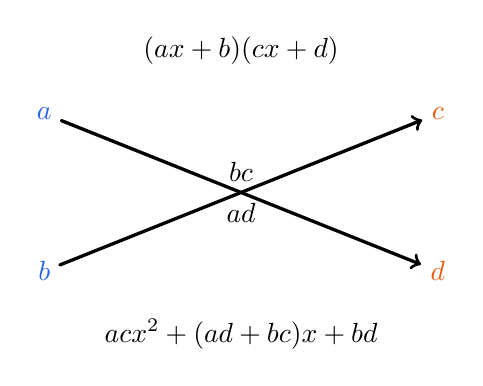
\begin{tikzpicture}[line cap=round,line join=round]
  \node[FigureBlue] (a) at (0,2) {$a$}; \node[FigureBlue] (b) at (0,0) {$b$};
  \node[FigureOrange] (c) at (5,2) {$c$}; \node[FigureOrange] (d) at (5,0) {$d$};
  \draw[->,line width=1.2pt] (a)--(d) node[midway,below] {$ad$};
  \draw[->,line width=1.2pt] (b)--(c) node[midway,above] {$bc$};
  \node at (2.5,2.8) {$(ax+b)(cx+d)$};
  \node at (2.5,-.8) {$acx^2+(ad+bc)x+bd$};
\end{tikzpicture}
\end{document}
